\documentclass{beamer}
\setbeamertemplate{navigation symbols}{}

\usepackage{beamerthemeshadow}
\usepackage{graphicx}
\usepackage{url}
\usepackage{listings}

\begin{document}
\title{Stackbased Languages}
\author[Serap Kadam \and Christoph M{\"u}llner]{Serap Kadam \and Christoph M{\"u}llner \\
$<$serapkadam@gmail.com$>$, $<$christophm30@gmail.com$>$}
\subtitle{Knight's Tour}

\date{\today} 

\begin{frame}
\titlepage
\end{frame}

\begin{frame}
\frametitle{Table of contents}
\tableofcontents
\end{frame} 

\section{Knight's tour} 
\begin{frame}
\frametitle{The problem}
"The Knight's Tour is a mathematical problem involving a knight
on a chessboard. The knight is placed on the empty board and,
moving according to the rules of chess, must visit each square
exactly once. 

A knight's tour is called a closed tour if the
knight ends on a square attacking the square from which it began.
Otherwise the tour is open." from wikipedia 

In German this problem is called "Springerproblem".

\end{frame}

\begin{frame}
\frametitle{Variations of the knight's problem}
 Knight's problem is an instance of the Hamiltonian path problem (NP-complete)
 
 Knight's Tour can be found in linear time!
\begin{itemize}
	\item Find a path for a given start and/or end position
	\item Find a closed path for a given position 
	\item Find a path for a board of size $n x m$ other than $8x8$
\end{itemize}
\end{frame}

\subsection{Background}
\begin{frame}
\frametitle{The knight and his movement}
\begin{figure}
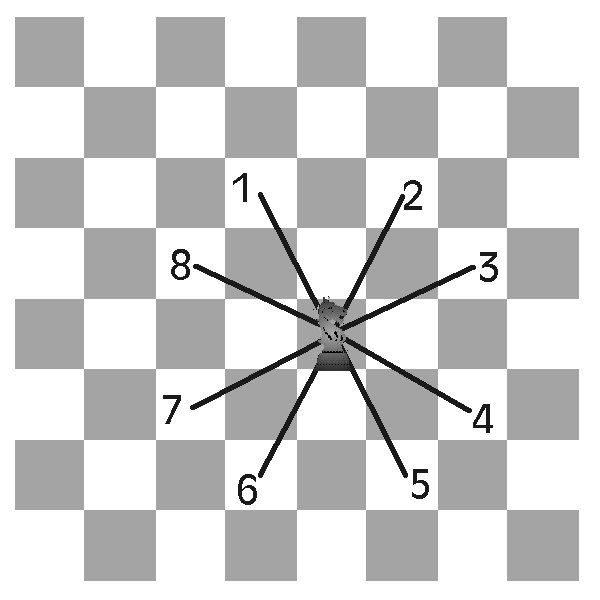
\includegraphics[scale=0.25]{sprung}
\caption{Possible moves of a knight}
\end{figure}
\end{frame}

\begin{frame}
\frametitle{One of many solutions}
\begin{figure}
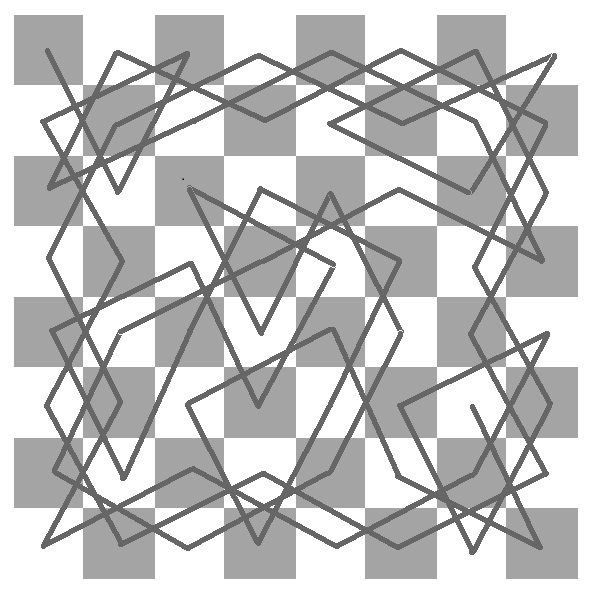
\includegraphics[scale=0.4]{loesung}
\caption{Possible solution on a $8x8$ chessboard}
\end{figure}
\end{frame}

\begin{frame}
\frametitle{An invalid solution}
\begin{figure}
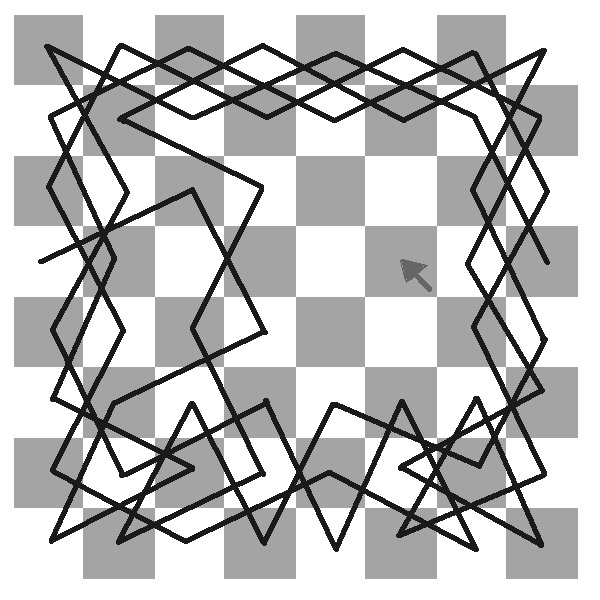
\includegraphics[scale=0.4]{luecke}
\caption{The marked square can't be reached anymore}
\end{figure}
\end{frame}

\subsection{Solutions}
\begin{frame}
\frametitle{Backtracking}
\begin{itemize}
	\item Choose a random path of unvisited positions
	\item If a dead end is reached $\rightarrow$ go back one step and
	continue with another position than the last chosen 
\end{itemize}
Always finds a solution, if there is one 
 
Slow! Better solution?
\end{frame}

\begin{frame}
\frametitle{Warnsdorff's algorithm}
Found by H. C. Warnsdorff (1823)\par
\begin{itemize}
	\item As long as there are reachable positions: visit unvisited position,
	which has the fewest successor positions
	\item Two positions with the same amount of successors $\rightarrow$
	choose any of these positions
	\item Only a (very good) heuristic $\rightarrow$ must not find a solution
	\item Even with board size $8x8$ there might be no solution
\end{itemize}

But: there are 13.267.364.410.532 undirected closed path solutions for a $8x8$ board

 $\rightarrow$ better heuristics 

\end{frame}

\begin{frame}
\frametitle{Extended solution}
\begin{itemize}
	\item For bigger boards: Divide \& Conquer
	\item $\forall n \geq 18, n, x, y, z \in \mathbb N, n = x*6 + y*7 + z * 8$
\end{itemize}

\begin{figure}
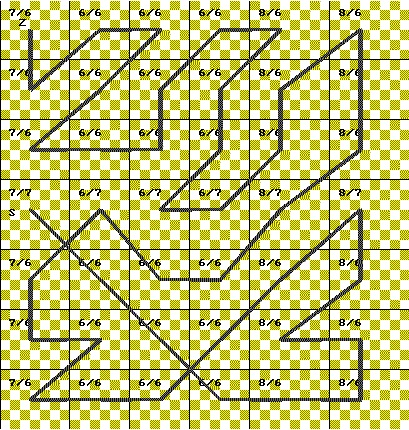
\includegraphics[scale=0.35]{spripic1}
\caption{Divide big board in smaller fields of size 6x6, 6x7, 6x8, 7x7, 7x8, 8x8
	and solve each field with a given start and end position, so that every subboard
	can be reached}
\end{figure}


\end{frame}


\section{Implementation}
\subsection{Language, task description}
\begin{frame}
\frametitle{Language and task description}
\begin{itemize}
	\item Language: PostScript (Ghostscipt), because of possible drawing
	\item Input: Start/end position of knight
	\item Output: Path of knight to end position
	\item Completeness for $8 x 8$ boards is desirable
\end{itemize}
\end{frame}

\subsection{Status and implementation details}
\begin{frame}
\frametitle{Algorithm}
\begin{enumerate}
	\item Start position on stack
	\item Put possible neighbours on stack
	\item Exit if no neighbours are reachable
	\item Pick best neighbour and drop the others
	\item Goto 2
\end{enumerate}
\end{frame}

\subsection{Open problems}
\begin{frame}
\frametitle{Problems, TODOs}
\begin{itemize}
	\item Usage of array for visited positions (any ideas?)
	\item Usage of 'count +1/-1 roll' (is this expensive?)
	\item Completeness for $8 x 8$ boards
\end{itemize}
\end{frame}

\section{Summary}
\begin{frame}
\frametitle{Summary}
\begin{itemize}
	\item Knight's problem
	\item Impementation
	\item Now: demonstration :)
\end{itemize}
\end{frame}

\end{document}
